
\documentclass[draft]{agujournal2019}
\usepackage{url} %this package should fix any errors with URLs in refs.
\usepackage{lineno}
\usepackage[inline]{trackchanges} %for better track changes. finalnew option will compile document with changes incorporated.
\usepackage{soul}
\linenumbers


\draftfalse


\journalname{Journal of Advances in Modeling Earth Systems (JAMES)}


\begin{document}


\title{The Community Land Model, version 5: \\ Parameter Perturbation Experiment}


%%%%%%%%%%%%%%%%%%%%%%%%%%%%%%%%%%%%%%%%%%%%%%%
%
%  AUTHORS AND AFFILIATIONS
%
%%%%%%%%%%%%%%%%%%%%%%%%%%%%%%%%%%%%%%%%%%%%%%%

% Authors are individuals who have significantly contributed to the
% research and preparation of the article. Group authors are allowed, if
% each author in the group is separately identified in an appendix.)

% List authors by first name or initial followed by last name and
% separated by commas. Use \affil{} to number affiliations, and
% \thanks{} for author notes.
% Additional author notes should be indicated with \thanks{} (for
% example, for current addresses).

% Example: \authors{A. B. Author\affil{1}\thanks{Current address, Antartica}, B. C. Author\affil{2,3}, and D. E.
% Author\affil{3,4}\thanks{Also funded by Monsanto.}}

\authors{Daniel Kennedy\affil{1}, Katherine Dagon\affil{1}, David M. Lawrence\affil{1}}


\affiliation{1}{Climate and Global Dynamics Laboratory, National Center for Atmospheric Research, Boulder, CO, USA}


\correspondingauthor{Daniel Kennedy}{djk2120@ucar.edu}



\begin{keypoints}
\item enter point 1 here
\item enter point 2 here
\item enter point 3 here
\end{keypoints}



\begin{abstract}
[ enter your Abstract here ]
\end{abstract}



\section{Introduction}
\section{Experiment description}


\subsection{Sparse grid}

Multivariate spatiotemporal clustering 

\begin{figure}[h]
\centering
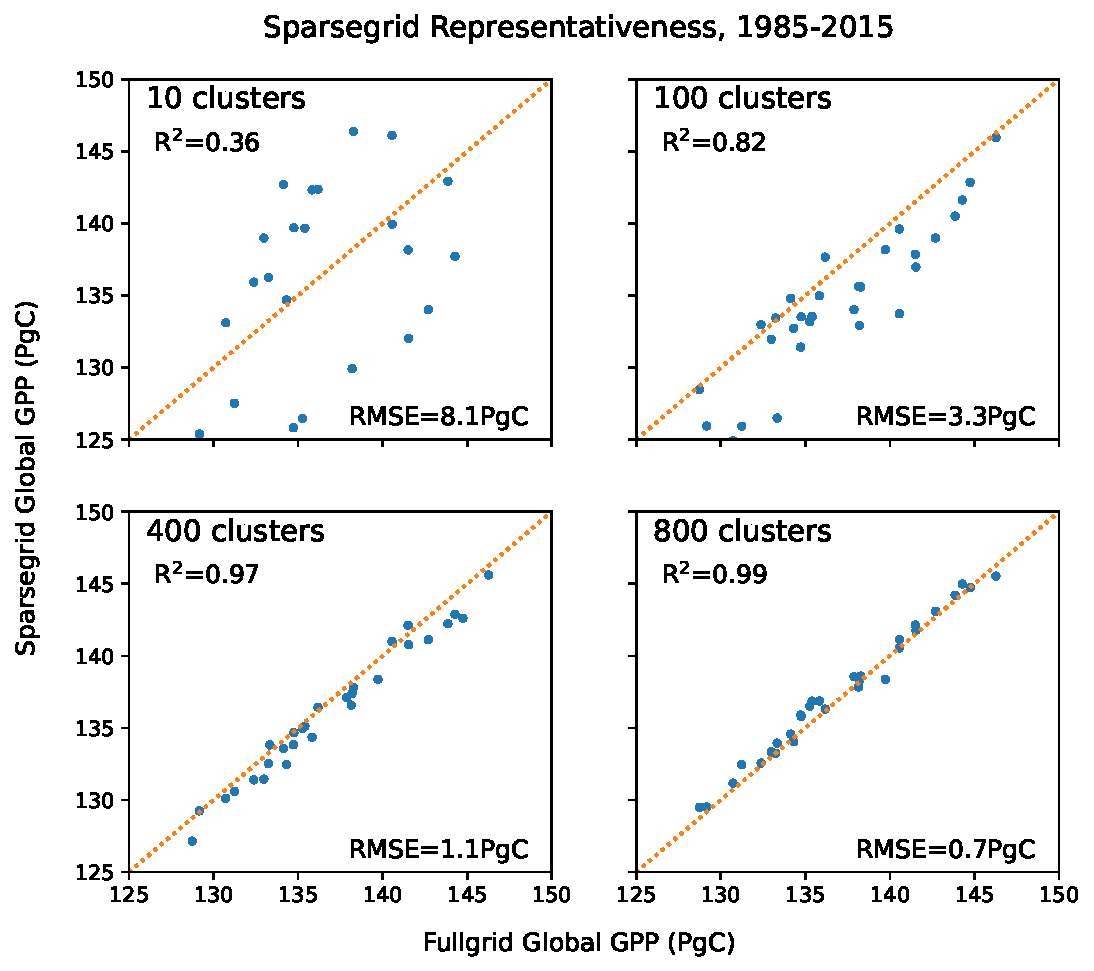
\includegraphics[width=40pc]{../figs/sparsegrid_gpp.pdf}
\caption{Sparsegrid vs fullgrid (2$^{\circ}$ resolution) global annual GPP across the last thirty years of a transient CLM5.1 simulation. We opted for 400 clusters (i.e. 400 sparse gridcells) to balance computational cost against representativeness. For reference there are 22,648 and 5,666 land gridcells in standard 1$^{\circ}$ and 2$^{\circ}$ CLM simulations, respectively.}
\label{fig:sparsegrid}
\end{figure}


\begin{figure}[h]
\centering
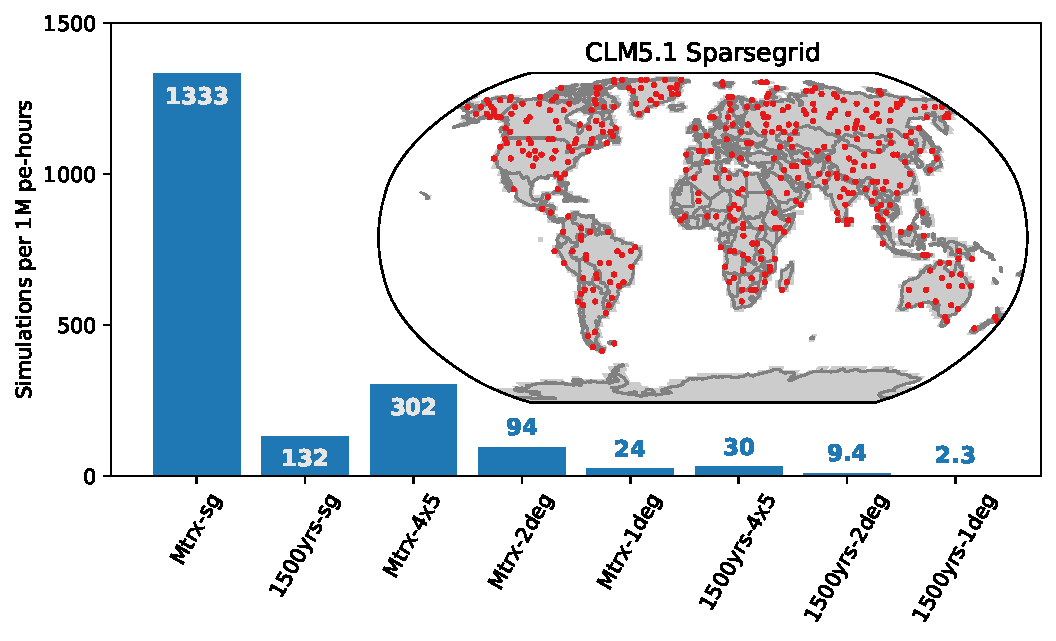
\includegraphics[width=25pc]{../figs/sims.pdf}
\caption{A standard 1-degree CLM-BGC simulation with 1500 years of spinup is prohibitively expensive ($\sim$400k pe-hours) for exhaustive parameter sensitivity testing. Utilizing the Matrix-CN spinup method and our sparsegrid configuration yields approximately 1300 simulations per million pe-hours.}
\label{fig:timing}
\end{figure}


\subsection{Forcing Scenarios}
\label{sect:exps}
 \begin{table}[h]
 \caption{Forcing Scenarios}
 \centering
 \begin{tabular}{l c c c c}
 \hline
  Name  & Meteorology & CO$_2$ (ppmv) & N addition & Description \\
 \hline
   CTL2010  & 2005-2014 & 367 & - & control experiment\\
   C285        & 2005-2014 & 285 & - & low CO$_2$ \\
   C867        & 2005-2014 & 867 & - & high CO$_2$ \\
   AF1855    & 1851-1860 & 367 & - & pre-industrial climate \\
   AF2095    & 2091-2100 & 367 & - & late century climate (SSP3-7.0) \\
   NDEP      & 2005-2014 & 367 & 5g/m$^2$ & enhanced nitrogen deposition \\
 \hline
 \end{tabular}
 \label{tab:exps}
 \end{table}



\break
\section{Results}


\begin{figure}[h]
\centering
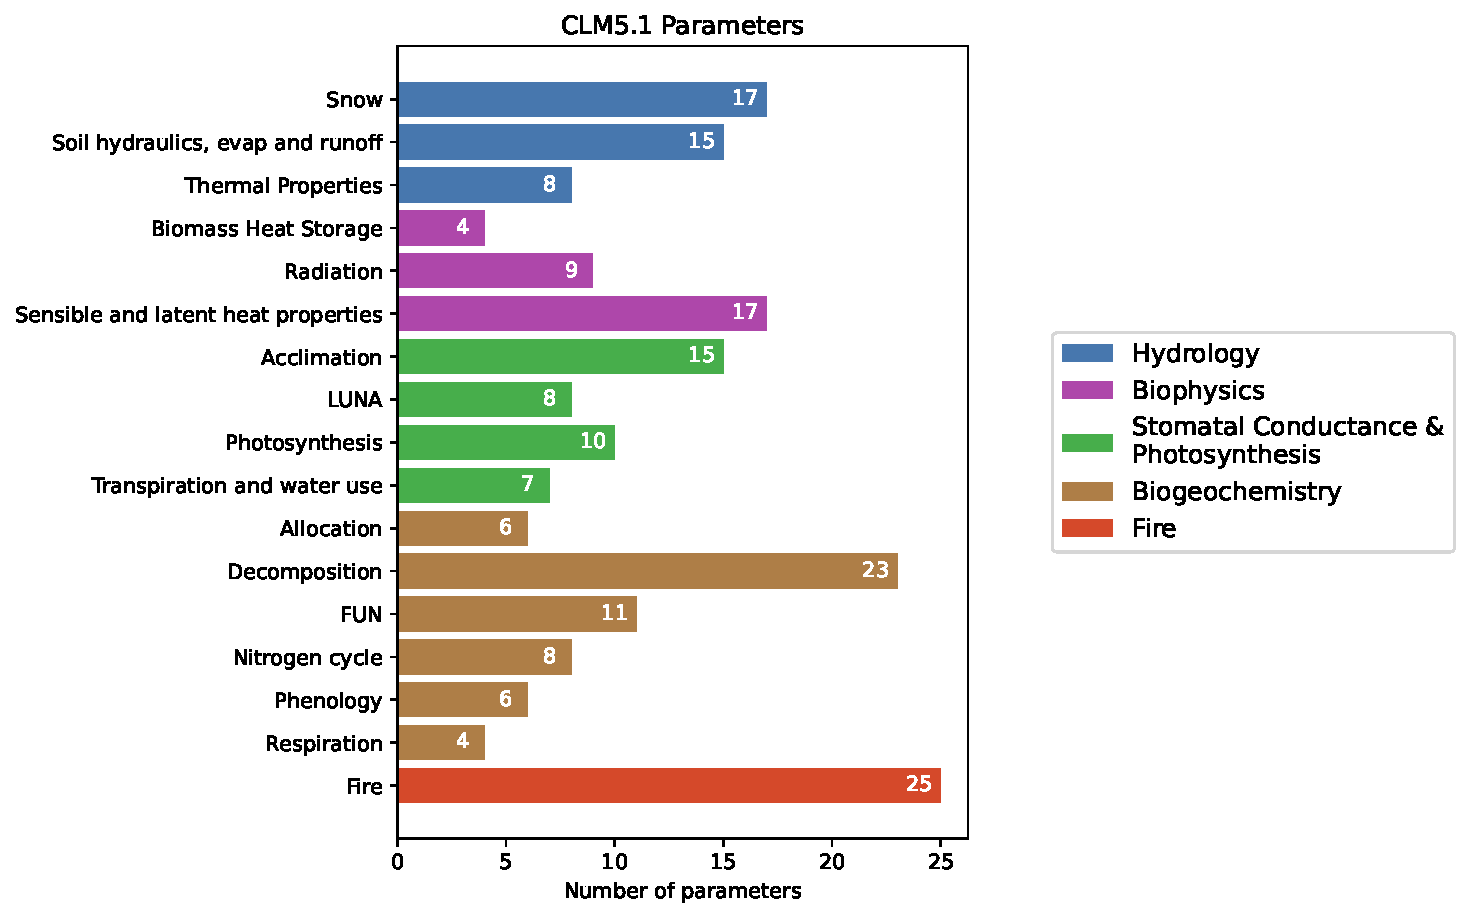
\includegraphics[width=30pc]{../figs/bar.pdf}
\caption{206 parameters were identified and perturbed across the various domains of the land model.}
\label{fig:params}
\end{figure}

\break

\begin{figure}[h]
\centering
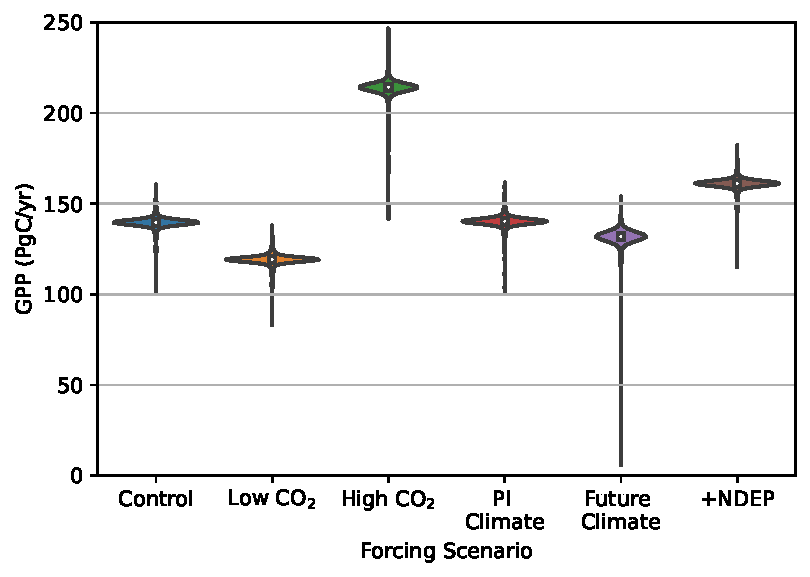
\includegraphics[width=25pc]{../figs/gpp_violin.pdf}
\caption{Distributions of global annual GPP across the six forcing scenarios. See Section \ref{sect:exps} for scenario descriptions.}
\label{fig:gpp1}
\end{figure}



\break

\begin{figure}[h]
\centering
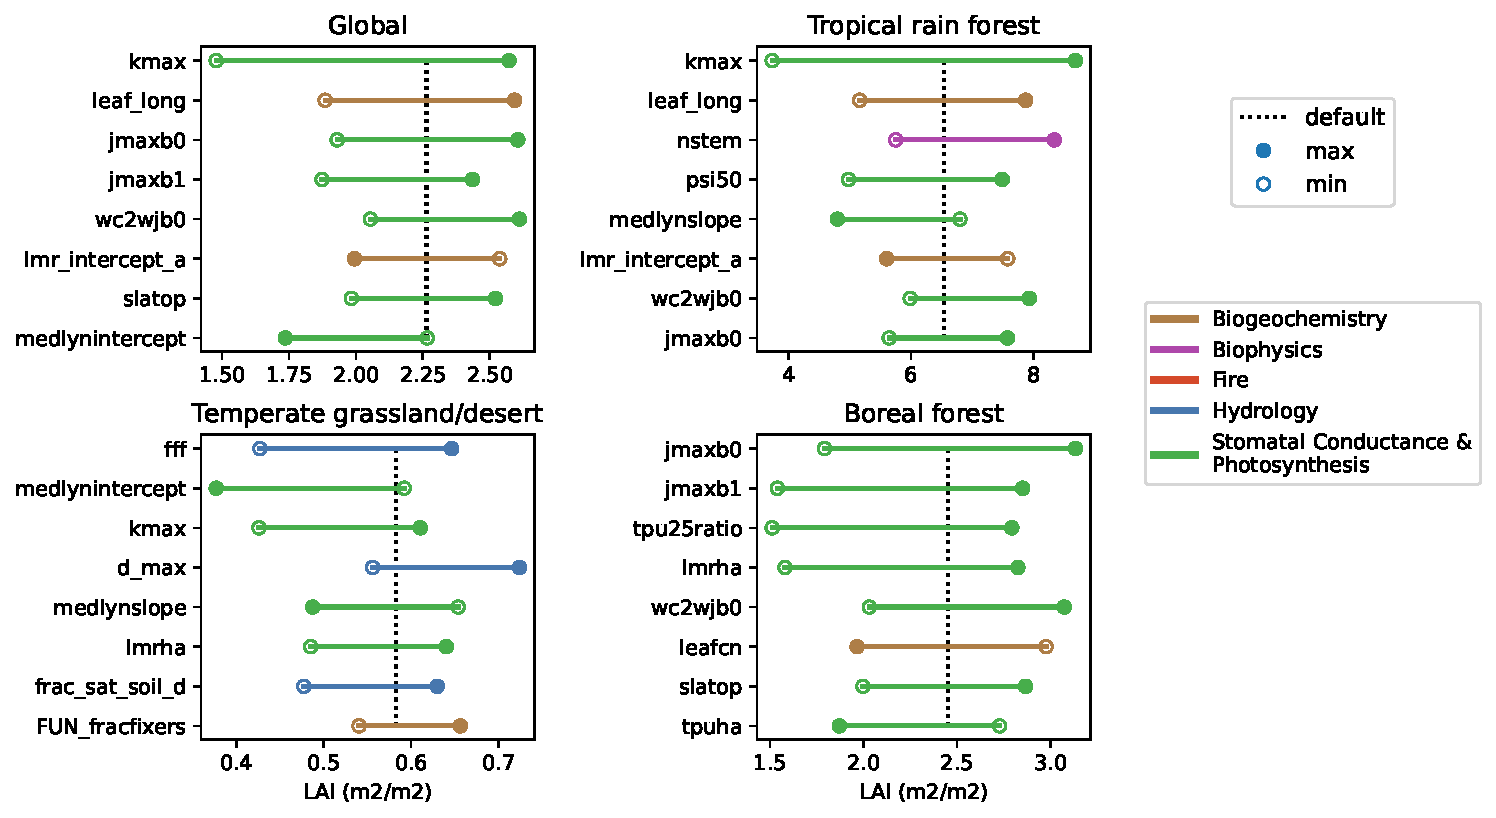
\includegraphics[width=40pc]{../figs/lai_biome.pdf}
\caption{The eight most influential parameters on leaf area index within the CTL2010 ensemble, globally and within three biomes.}
\label{fig:lai}
\end{figure}



\break



\begin{figure}[h]
\centering
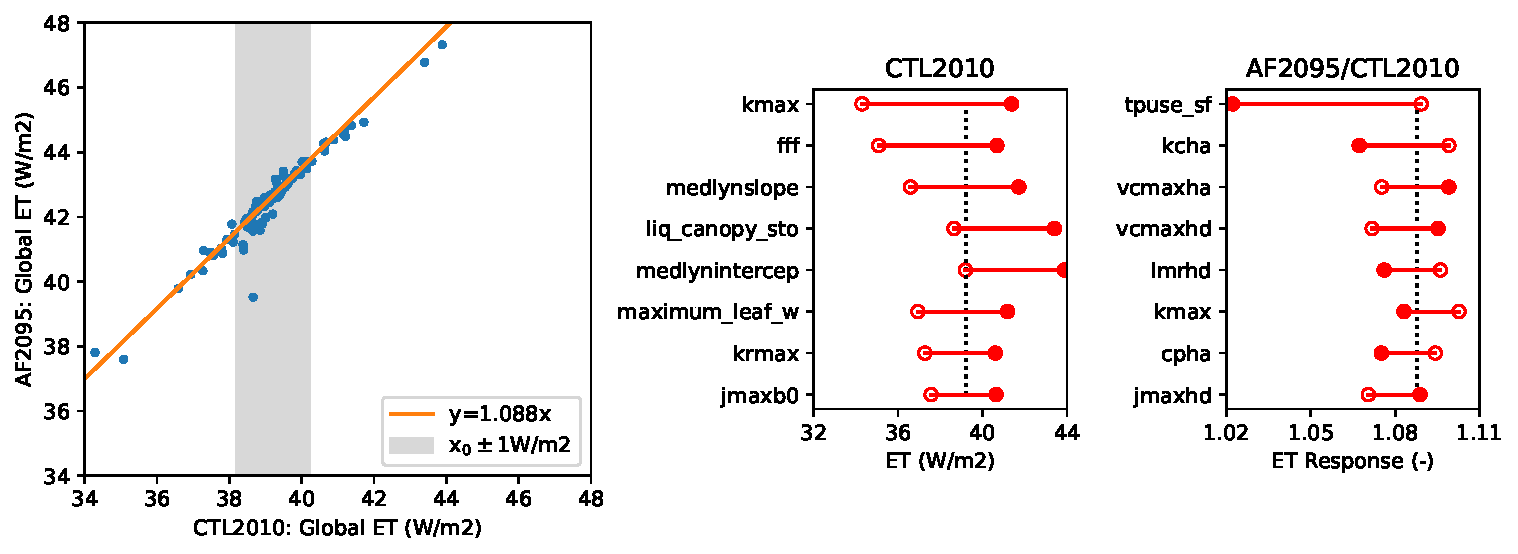
\includegraphics[width=40pc]{../figs/ET_response.pdf}
\caption{(a) Global evapotranspiration in the warm forcing scenario vs. our control experiment. The default parameterization ET enhancement is +8.8\%, as shown with the orange line. The shading spans the CTL2010 default ET, plus or minus 1 W/m2.
(b) The top 8 parameters governing global ET in the CTL2010 experiment.
(c) The top 8 parameters governing ET response to the future climate anomaly forcing (AF2095).
Parameters governing the response to temperature anomalies tend to differ from the parameters controlling present-day ET.}
\label{fig:et}
\end{figure}

\break

\begin{figure}[h]
\centering
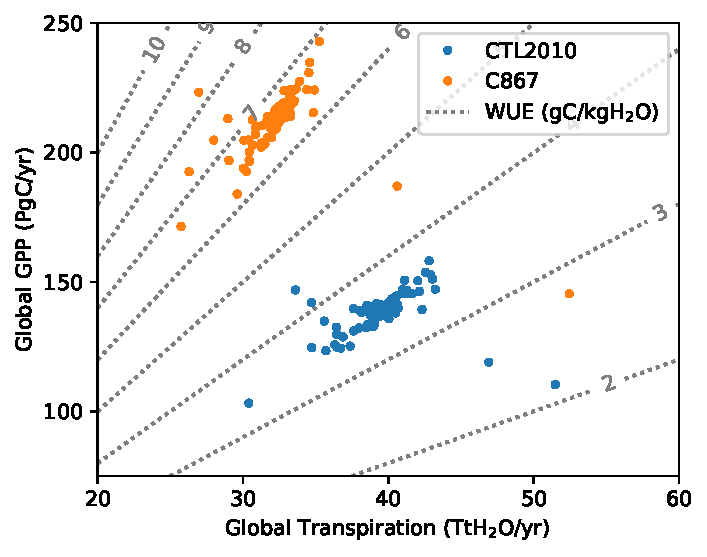
\includegraphics[width=25pc]{../figs/wue.pdf}
\caption{Global photosynthesis vs. transpiration for the control and high CO$_2$ ensembles. Water use efficiency (in this case defined as GPP/T) contours are drawn for reference. The default parameterization increases GPP by 53\% in response to increasing CO$_2$ from 367 to 867 ppm, made possible by an even larger increase in WUE (+88\%).}
\label{fig:wue}
\end{figure}




\break

\begin{figure}[h]
\centering
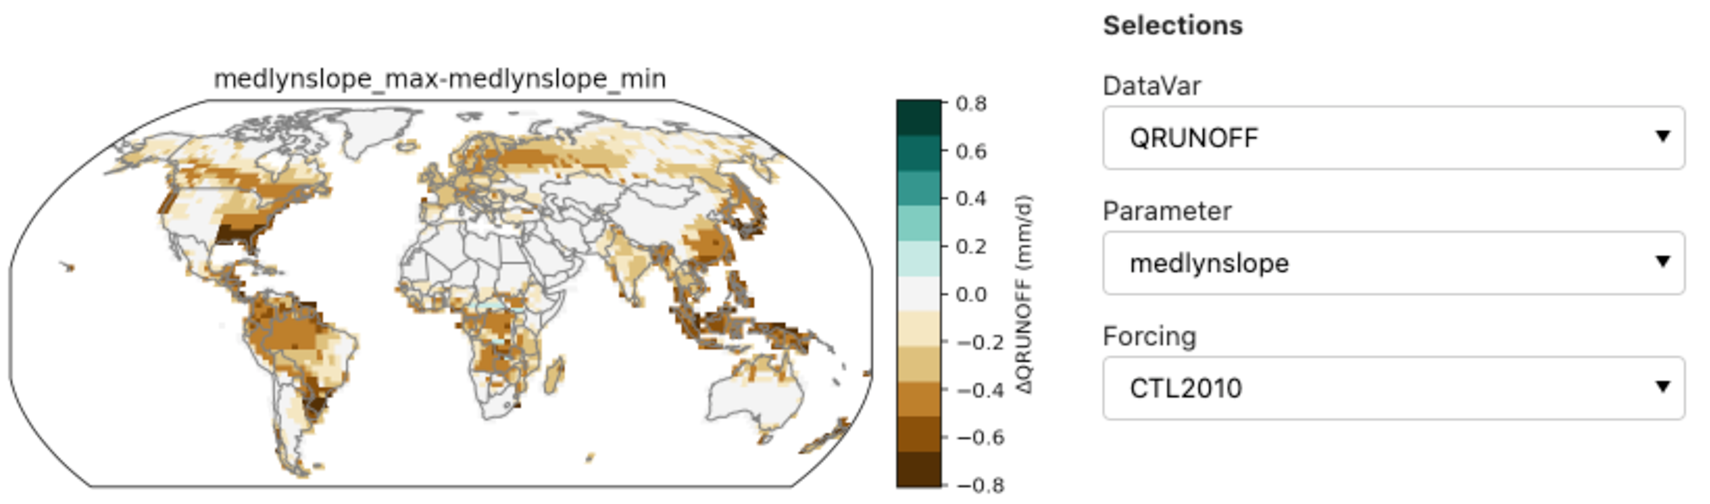
\includegraphics[width=40pc]{../figs/deltmap_panel.pdf}
\caption{Screenshot of interactive diagnostic for exploring maps of parameter effects. In this case, the effect of medlynslope on runoff within the CTL2010 ensemble. Increasing medlynslope tends to increase transpiration and reduce runoff.}
\label{fig:panel}
\end{figure}


\break




%%%%%%%%%%%%%%%%%%%%%%%%%%%%%%%%%%%%%%%%%%%%%%%
% REFERENCES and BIBLIOGRAPHY
%
% \bibliography{<name of your .bib file>} don't specify the file extension
% don't specify bibliographystyle
%
%%%%%%%%%%%%%%%%%%%%%%%%%%%%%%%%%%%%%%%%%%%%%%%

%\bibliography{ enter your bibtex bibliography filename here }



%Reference citation instructions and examples:
%
% Please use ONLY \cite and \citeA for reference citations.
% \cite for parenthetical references
% ...as shown in recent studies (Simpson et al., 2019)
% \citeA for in-text citations
% ...Simpson et al. (2019) have shown...
%
%
%...as shown by \citeA{jskilby}.
%...as shown by \citeA{lewin76}, \citeA{carson86}, \citeA{bartoldy02}, and \citeA{rinaldi03}.
%...has been shown \cite{jskilbye}.
%...has been shown \cite{lewin76,carson86,bartoldy02,rinaldi03}.
%... \cite <i.e.>[]{lewin76,carson86,bartoldy02,rinaldi03}.
%...has been shown by \cite <e.g.,>[and others]{lewin76}.
%
% apacite uses < > for prenotes and [ ] for postnotes
% DO NOT use other cite commands (e.g., \citet, \citep, \citeyear, \nocite, \citealp, etc.).
%



\end{document}



More Information and Advice:

%%%%%%%%%%%%%%%%%%%%%%%%%%%%%%%%%%%%%%%%%%%%%%%
%
%  SECTION HEADS
%
%%%%%%%%%%%%%%%%%%%%%%%%%%%%%%%%%%%%%%%%%%%%%%%

% Capitalize the first letter of each word (except for
% prepositions, conjunctions, and articles that are
% three or fewer letters).

% AGU follows standard outline style; therefore, there cannot be a section 1 without
% a section 2, or a section 2.3.1 without a section 2.3.2.
% Please make sure your section numbers are balanced.
% ---------------
% Level 1 head
%
% Use the \section{} command to identify level 1 heads;
% type the appropriate head wording between the curly
% brackets, as shown below.
%
%An example:
%\section{Level 1 Head: Introduction}
%
% ---------------
% Level 2 head
%
% Use the \subsection{} command to identify level 2 heads.
%An example:
%\subsection{Level 2 Head}
%
% ---------------
% Level 3 head
%
% Use the \subsubsection{} command to identify level 3 heads
%An example:
%\subsubsection{Level 3 Head}
%
%---------------
% Level 4 head
%
% Use the \subsubsubsection{} command to identify level 3 heads
% An example:
%\subsubsubsection{Level 4 Head} An example.
%
%%%%%%%%%%%%%%%%%%%%%%%%%%%%%%%%%%%%%%%%%%%%%%%
%
%  IN-TEXT LISTS
%
%%%%%%%%%%%%%%%%%%%%%%%%%%%%%%%%%%%%%%%%%%%%%%%
%
% Do not use bulleted lists; enumerated lists are okay.
% \begin{enumerate}
% \item
% \item
% \item
% \end{enumerate}
%
%%%%%%%%%%%%%%%%%%%%%%%%%%%%%%%%%%%%%%%%%%%%%%%
%
%  EQUATIONS
%
%%%%%%%%%%%%%%%%%%%%%%%%%%%%%%%%%%%%%%%%%%%%%%%

% Single-line equations are centered.
% Equation arrays will appear left-aligned.

Math coded inside display math mode \[ ...\]
 will not be numbered, e.g.,:
 \[ x^2=y^2 + z^2\]

 Math coded inside \begin{equation} and \end{equation} will
 be automatically numbered, e.g.,:
 \begin{equation}
 x^2=y^2 + z^2
 \end{equation}


% To create multiline equations, use the
% \begin{eqnarray} and \end{eqnarray} environment
% as demonstrated below.
\begin{eqnarray}
  x_{1} & = & (x - x_{0}) \cos \Theta \nonumber \\
        && + (y - y_{0}) \sin \Theta  \nonumber \\
  y_{1} & = & -(x - x_{0}) \sin \Theta \nonumber \\
        && + (y - y_{0}) \cos \Theta.
\end{eqnarray}

%If you don't want an equation number, use the star form:
%\begin{eqnarray*}...\end{eqnarray*}

% Break each line at a sign of operation
% (+, -, etc.) if possible, with the sign of operation
% on the new line.

% Indent second and subsequent lines to align with
% the first character following the equal sign on the
% first line.

% Use an \hspace{} command to insert horizontal space
% into your equation if necessary. Place an appropriate
% unit of measure between the curly braces, e.g.
% \hspace{1in}; you may have to experiment to achieve
% the correct amount of space.


%%%%%%%%%%%%%%%%%%%%%%%%%%%%%%%%%%%%%%%%%%%%%%%
%
%  EQUATION NUMBERING: COUNTER
%
%%%%%%%%%%%%%%%%%%%%%%%%%%%%%%%%%%%%%%%%%%%%%%%

% You may change equation numbering by resetting
% the equation counter or by explicitly numbering
% an equation.

% To explicitly number an equation, type \eqnum{}
% (with the desired number between the brackets)
% after the \begin{equation} or \begin{eqnarray}
% command.  The \eqnum{} command will affect only
% the equation it appears with; LaTeX will number
% any equations appearing later in the manuscript
% according to the equation counter.
%

% If you have a multiline equation that needs only
% one equation number, use a \nonumber command in
% front of the double backslashes (\\) as shown in
% the multiline equation above.

% If you are using line numbers, remember to surround
% equations with \begin{linenomath*}...\end{linenomath*}

%  To add line numbers to lines in equations:
%  \begin{linenomath*}
%  \begin{equation}
%  \end{equation}
%  \end{linenomath*}



